\documentclass[16pt]{article}
\usepackage[english]{babel}
\usepackage{longtable}
\usepackage[top=1in, bottom=0.25in, left=1.25in, right=1.25in,includefoot,heightrounded]{geometry}
\usepackage{indentfirst}
\usepackage[utf8]{inputenc}
\usepackage{amsmath,amssymb}
\usepackage{graphicx,tikz}
\usepackage{hyperref}
\usepackage[colorinlistoftodos]{todonotes}
\usepackage[document]{ragged2e}
\usepackage{fancyhdr}
\usepackage{enumerate}
\usepackage{listings}
\usepackage{color}
\usepackage{flowchart}
\usepackage{hyperref}
\usepackage{graphicx}
\usetikzlibrary{arrows}


\usetikzlibrary{shapes.geometric, arrows}
\tikzstyle{startstop} = [rectangle, rounded corners, minimum width=3cm, minimum height=1cm,text centered, draw=black, fill=red!30]
\tikzstyle{decision} = [diamond, minimum width=4cm, minimum height=0.5cm, text centered, draw=black, fill=green!30]
\tikzstyle{process} = [rectangle, minimum width=3cm, minimum height=1cm, text centered, draw=black, fill=orange!30]
\tikzstyle{arrow} = [thick,->,>=stealth]
\tikzstyle{io} = [trapezium, trapezium left angle=70, trapezium right angle=110, minimum width=2cm, text width=4cm, minimum height=1cm, text centered, draw=black, fill=blue!30]

\pagestyle{fancy}
\fancyhf{}
\lhead{Myles Deslippe}
\rhead{Comp 3670 | Computer Networks}
\cfoot{\thepage}

\definecolor{MyDarkGreen}{rgb}{0.0,0.4,0.0}
\lstset{inputencoding=ansinew}
\lstset{breaklines=true} 

\begin{document}

    \section*{\centering{Network Applications}}

    \subsection*{Principals of Network Applications}
    \begin{itemize}
        \item To create a \textbf{network application}, we need to write a program that runs on \textbf{different end systems}, and \textbf{communicates over a network}.
        \item There is a \textbf{layer of abstraction} between \textbf{network applications} and \textbf{the network}; allowing for \textbf{rapid network application development}.
        \item There are different \textbf{application architectures} we can use to developer \textbf{network applications}.
    \end{itemize}

    \subsection*{Client-Server Architecture}
    \begin{itemize}
        \item The \textbf{client-server architecture} consists of two entities, the \textbf{client} and the \textbf{server}.
        \item The \textbf{sever} is a \textbf{network host that is always on}, and has a \textbf{permanent IP address}.
        \item The \textbf{client} communicate with the \textbf{server} over a \textbf{network}, and can have a \textbf{dynamic IP address}.
        \item The clients do not \textbf{directly communicate}, they use the \textbf{server to communicate}.
    \end{itemize}

    \subsection*{Peer to Peer Architecture}
    \begin{itemize}
        \item The \textbf{peer to peer architecture} has \textbf{no always-on server}.
        \item The \textbf{clients communicate directly}.
    \end{itemize}

    \subsection*{Process Communication}
    \begin{itemize}
        \item A \textbf{process} is a \textbf{program running on a network host}.
        \item \textbf{Processes} in the \textbf{same host} use \textbf{inter-process communication} to communicate.
        \item \textbf{Processes} in \textbf{different hosts} use \textbf{network-communication} to communicate.
        \item The \textbf{server process} is a process that \textbf{waits to be contacted by clients}.
        \item The \textbf{client process} is a process that \textbf{initiates communication with the server}.
    \end{itemize}

    \subsection*{Sockets}
    \begin{itemize}
        \item One way \textbf{two process} can \textbf{connect over a network} is with \textbf{sockets}.
        \item A \textbf{socket} is a \textbf{structure within a network host} that \textbf{serves as an endpoint} for \textbf{sending and receiving data}.
        \item In order for \textbf{network hosts to communicate}, they must each have a \textbf{unique Internet Protocol Address (IP Address)}.
        \item The \textbf{operating system} uses the \textbf{ports} of the \textbf{server and client} to make sure the information ends up in the \textbf{correct place}.
    \end{itemize}

    \subsection*{Application Layer Protocols}
    \begin{itemize}
        \item \textbf{Application Layer Protocols} define how \textbf{application processes} running on \textbf{different end systems communicate}.
        \item The \textbf{protocols} define \textbf{the message syntax, semantics, and rules}.
        \item The \textbf{type of transport} an \textbf{application} uses depends on what is \textbf{important to the application}; such as \textbf{data integrity, throughput, timing, etc}.
    \end{itemize}

    \subsection*{Internet Transport Services}
    \begin{itemize}
        \item There are \textbf{two internet transport protocol services}:
        \begin{enumerate}
            \item \textbf{User Datagram Protocol (UDP)} is a \textbf{transport protocol} that is \textbf{fast but unreliable}. UDP has \textbf{no confirmation} that the \textbf{packets were delivered}; upd is \textbf{not connection-oriented}.
            \item \textbf{Transport Control Protocol (TCP)} is a \textbf{transport protocol} that is \textbf{reliable, but has more overhead}. TCP has \textbf{flow control, congestion control, and is connection oriented}.
        \end{enumerate}
        \item \textbf{TCP and UDP} have \textbf{no encryption} by default.
        \item To \textbf{secure data} being transferred with \textbf{TCP} we use a \textbf{Secure Socket Layer (SSL)} which provides \textbf{encryption, data integrity, and end-point authentication}.
        \begin{itemize}
            \item \textbf{SSL} is a part of the \textbf{application-layer}.
        \end{itemize}
    \end{itemize}

    \section*{\centering{The World Wide Web}}

    \subsection*{Introduction}
    \begin{itemize}
        \item The \textbf{Word Wide Web or Web} is the world's dominant \textbf{software platform}.
        \item The \textbf{web} is an information space where \textbf{documents and other resources} can be \textbf{accessed through the internet} using a \textbf{web browser}.
        \item A \textbf{web page} is a \textbf{hypertext document} that is delivered by a \textbf{web server}.
        \item A \textbf{website} consists of \textbf{many webpages} linked together under a common \textbf{host}.
        \item \textbf{Web resources} can be accessed through a \textbf{Uniform Resource Locator (URL)}.
        \item[] 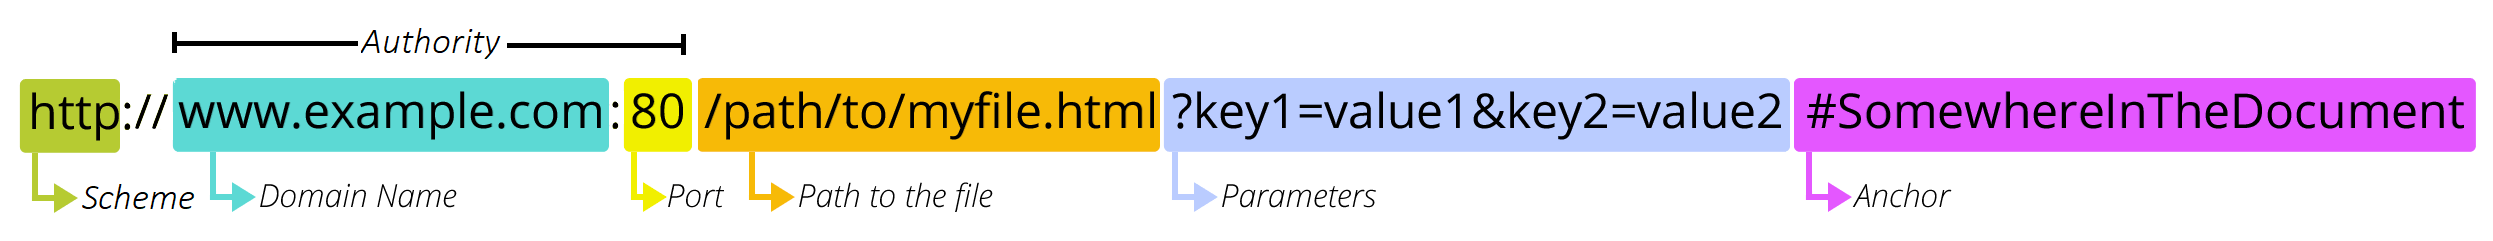
\includegraphics[width=407px]{images/URL.png}
    \end{itemize}
    
    \subsection*{Hypertext Transfer Protocol}
    \begin{itemize}
        \item The \textbf{web} uses the \textbf{Hypertext Transfer Protocol (HTTP) suite} to transfer data over the \textbf{internet}.
            \item \textbf{HTTP} uses \textbf{TCP} to facilitate the actual data transfer as follows:
            \begin{enumerate}
                \item The \textbf{client} initiates the \textbf{TCP} connection with the \textbf{server} (typically on port 80).
                \item The \textbf{server} accepts the \textbf{TCP} connection from the \textbf{client}.
                \item \textbf{HTTP messages} are exchanged between the \textbf{browser} and the \textbf{server}.
                \item The \textbf{TCP} connection is \textbf{closed}.
            \end{enumerate}
        \item \textbf{HTTP} is \textbf{stateless}.
        \item There are \textbf{two} types of \textbf{HTTP connections}:
        \begin{enumerate}
            \item \textbf{Persistent HTTP} is a connection where multiple files can be sent over a \textbf{single TCP connection} between the \textbf{client} and the \textbf{server}.
            \item \textbf{Non-Persistent HTTP} is where each file requires a \textbf{separate TCP connection} between the \textbf{client} and the \textbf{server}. 
        \end{enumerate}

    \end{itemize}

    \subsection*{Hypertext Transfer Protocol Requests}
    \begin{itemize}
        \item \textbf{HTTP requests} are the \textbf{messages} used to communicate over the \textbf{HTTP protocol}.
        \item There are \textbf{two main parts} of the request:
        \begin{enumerate}
            \item \textbf{The Header} is the field of an \textbf{HTTP request or response} that passes \textbf{additional context and metadata} about the request.
            \item \textbf{The Body} is the field of an \textbf{HTTP request or response} that passes the \textbf{target data}.
        \end{enumerate}
        \item There are two \textbf{8 types of HTTP request methods}:
        \begin{enumerate}
            \item The \textbf{GET method} is used to \textbf{retrieve information} from the server.
            \item The \textbf{HEAD method} is used to \textbf{retrieve information} from the server, but it transfers the status line and the header only.
            \item The \textbf{POST method} is used to \textbf{send data} to the server.
            \item The \textbf{PUT method} is used to \textbf{replace data} on the server.
            \item The \textbf{DELETE method} is used to \textbf{delete data} on the server.
            \item The \textbf{CONNECT method} is used to \textbf{establish a tunnel to the server}.
            \item The \textbf{OPTIONS method} is used to \textbf{describe the communication options} for the target resource.
            \item The \textbf{TRACE method} is used to \textbf{perform a message loop back test}.
        \end{enumerate}
    \end{itemize}
    
    \subsection*{Maintaining State over HTTP}
    \begin{itemize}
        \item Since \textbf{HTTP requests have no state}, we use \textbf{cookies}.
        \item \textbf{Cookies} are \textbf{key-value pairs} that are \textbf{sent back-and-forth with each request} (similar to headers).
    \end{itemize}

    \subsection*{Web Cache (Proxy Servers)}
    \begin{itemize}
        \item ISPs will use \textbf{cache proxy servers} to serve \textbf{cached data}, to lessen the load on the \textbf{origin server}.
        \item If the data is \textbf{not found on the cache proxy server}, the request will be \textbf{forwarded to the origin server}.
        \item \textbf{Cache servers} can reduce the response time for requests, and reduce the traffic on access links.
    \end{itemize}

\end{document}